\chapter{Diseño Y Prototipado} \label{CapDiseño}

\section{Teclados, entendiendo sus partes}

En esta primera sección vamos a ver todas las partes de un teclado y que funciones tienen cada una de ellas. Además, como interactúan entre sí y qué opciones hay. \cite{TearDownImageSource} La estructura general de un teclado es la que se muestra en la figura \ref{fig:TearDown} que podemos, además, ver a continuación. Esta figuro muestra las diferentes partes que un teclado podría tener. Aunque es cierto que aquí se muestran muchas más de las necesarias y de las que se usan normalmente. Más adelante se expondrán las partes que se van a usar en el teclado del proyecto.

\begin{figure}[H]
    \centering
    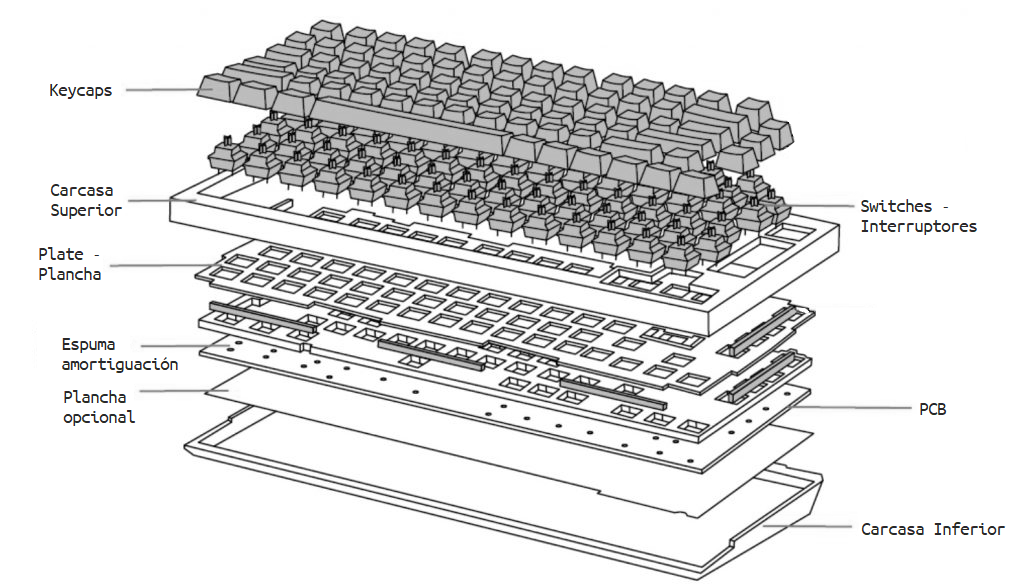
\includegraphics[width=1\textwidth]{imagenes/Capitulos/Cap03/KeyboardTeardown.png}
    \caption{Estructura física de un teclado \cite{TearDownImageSource}}
    \label{fig:TearDown}
\end{figure}



\subsubsection{\gls{Keycaps}}

Los \glsnocase{Keycaps} son las tapas individuales que cubren las teclas en un teclado. Estas tapas suelen estar hechas de plástico y están diseñadas para permitir que los usuarios escriban y presionen las teclas de manera cómoda y precisa. Podemos ver un ejemplo en la figura \ref{fig:Keycaps}. Los \glsnocase{Keycaps} pueden variar en diseño, color, material y perfil, y algunos teclados personalizados incluso permiten a los usuarios intercambiar los \glsnocase{Keycaps} para personalizar la apariencia o mejorar la sensación táctil del teclado. Algunos entusiastas de los teclados también coleccionan \glsnocase{Keycaps} únicos y personalizados para crear conjuntos únicos y estéticamente atractivos. Para poder hacernos una idea de cómo son los \glsnocase{Keycaps} se muestra la figura \ref{fig:Keycaps}.

\begin{figure}[H]
    \centering
    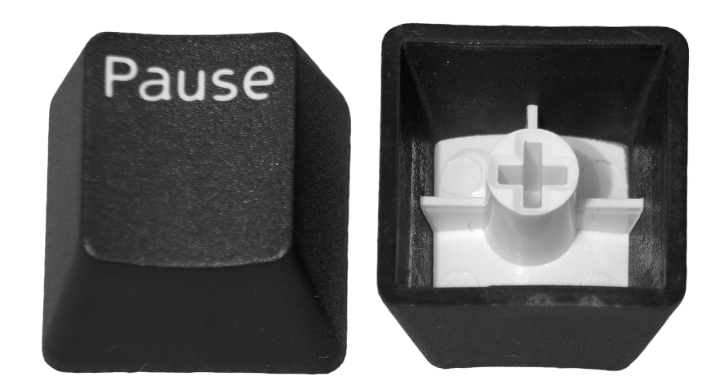
\includegraphics[width=0.75\textwidth]{imagenes/Capitulos/Cap03/Keycaps.png}
    \caption{\gls{Keycaps} \cite{KeycapsImageSource}}
    \label{fig:Keycaps}
\end{figure}

\subsubsection{\gls{Switches} o Interruptores}

Los \glsnocase{Switches} son los mecanismos debajo de cada tecla de un teclado que detectan cuándo se presiona una tecla y envían la señal al dispositivo electrónico al que está conectado el teclado. Estos \glsnocase{Switches} pueden variar significativamente en términos de sensación táctil, fuerza de actuación y ruido producido al presionar la tecla.

\begin{itemize}
  \item \textbf{\gls{Switches} de membrana}: Estos son los más comunes y se utilizan en muchos teclados estándar. Consisten en una membrana de goma debajo de las teclas que se comprime cuando se presiona una tecla, cerrando un circuito eléctrico y enviando una señal al dispositivo.
  
  \item \textbf{\gls{Switches} de tijera}: Estos \glsnocase{Switches} utilizan una estructura de tijera debajo de las teclas para proporcionar una sensación de escritura más estable y una mejor respuesta táctil que los \glsnocase{Switches} de membrana estándar.
  
  \item \textbf{\gls{Switches} mecánicos}: Son \glsnocase{Switches} individuales que utilizan un mecanismo mecánico para registrar la pulsación de una tecla. Hay varios tipos de \glsnocase{Switches} mecánicos, incluyendo los populares \glsnocase{Switches} Cherry MX, que vienen en variantes como los \glsnocase{Switches} lineales, táctiles y clicky, que ofrecen diferentes sensaciones táctiles y niveles de ruido. Para hacernos una idea de cómo serían estos \glsnocase{Switches} se muestra la figura \ref{fig:Switches}.
  
  \item \textbf{\gls{Switches} ópticos}: En lugar de utilizar contactos eléctricos, los \glsnocase{Switches} ópticos utilizan luz infrarroja para detectar cuando se presiona una tecla. Ofrecen una mayor durabilidad y una respuesta más rápida en comparación con los \glsnocase{Switches} mecánicos tradicionales.
\end{itemize}

\begin{figure}[H]
    \centering
    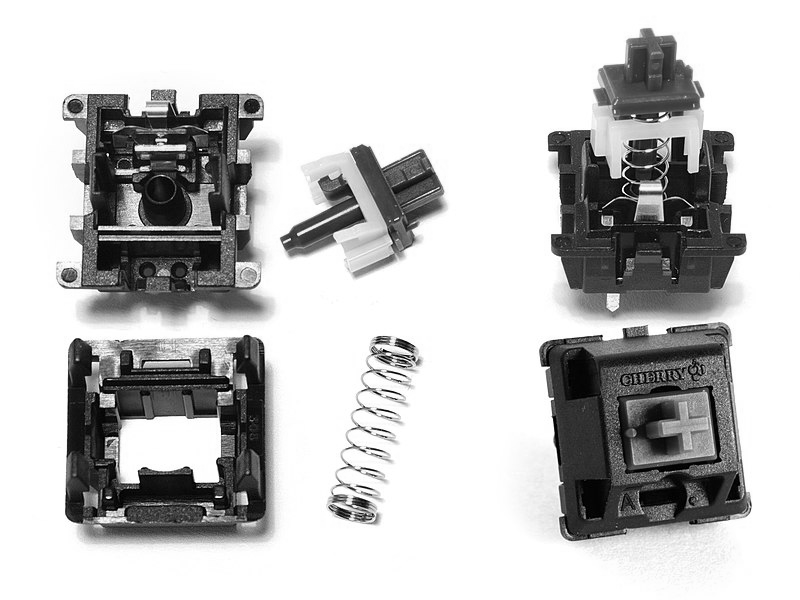
\includegraphics[width=1\textwidth]{imagenes/Capitulos/Cap03/Switches.png}
    \caption{Switches o Interruptores mecánicos \cite{SwitchesImageSource}}
    \label{fig:Switches}
\end{figure}

Los \glsnocase{Switches} son un componente clave en la experiencia de escritura de un teclado y pueden afectar la velocidad, la comodidad y la precisión al escribir. Los entusiastas de los teclados a menudo tienen preferencias personales sobre el tipo de \glsnocase{Switches} que prefieren, y algunos incluso personalizan sus teclados con \glsnocase{Switches} específicos para adaptarse a sus necesidades y preferencias individuales.
\newpage
\subsubsection{Carcasa superior}

La carcasa superior de un teclado es la parte que cubre la parte superior del teclado y proporciona la estructura externa. Esta carcasa puede variar en diseño y material según el tipo de teclado. En los teclados estándar, la carcasa superior suele estar hecha de plástico, mientras que en teclados de alta gama puede estar hecha de materiales más duraderos como aluminio o acero. La carcasa superior también puede incluir características adicionales, como reposamuñecas integrados o iluminación \gls{LED}, dependiendo del diseño y la funcionalidad del teclado. En nuestro caso vamos a combinar esta junto con la inferior para formar una combinada que proporciona soporte y estructura sin que tenga que ser otra pieza nueva. Un ejemplo de una carcasa de plástico se puede ver en la figura \ref{fig:TopCase1} y la respectiva carcasa volteada en la figura \ref{fig:TopCase2}.

\begin{figure}[H]
    \centering
    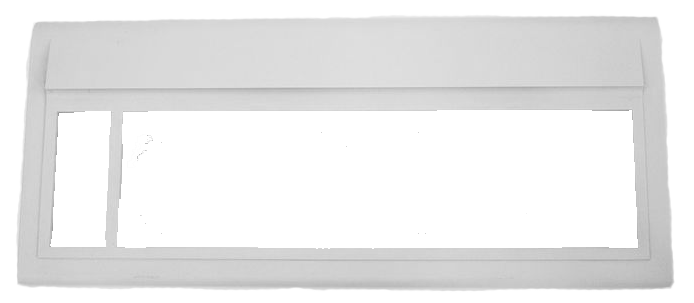
\includegraphics[width=1\textwidth]{imagenes/Capitulos/Cap03/TopCase2.png}
    \caption{Carcasa Superior \cite{TopCase2ImageSource}}
    \label{fig:TopCase2}
\end{figure}

\begin{figure}[H]
    \centering
    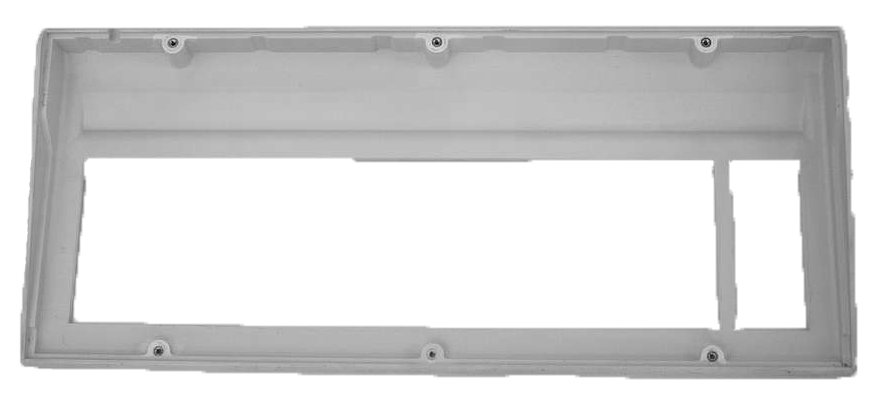
\includegraphics[width=1\textwidth]{imagenes/Capitulos/Cap03/TopCase1.png}
    \caption{Carcasa Superior Reverso \cite{TopCase1ImageSource}}
    \label{fig:TopCase1}
\end{figure}

\subsubsection{\gls{Plate} o Plancha} \label{DiseñoPlatePCB}

El \glsnocase{Plate}, también conocido como placa o plancha en español, es una pieza metálica o plástica que se coloca debajo de los \glsnocase{Switches} en un teclado mecánico. Su principal función es proporcionar soporte estructural a los \glsnocase{Switches} y distribuir uniformemente la fuerza ejercida al presionar las teclas sobre la superficie del teclado. Además, el \glsnocase{Plate} también influye en la sensación táctil y el sonido de las pulsaciones de las teclas.

La elección del material y diseño del \glsnocase{Plate} puede afectar la experiencia de escritura del usuario. Por ejemplo, los \glsnocase{Plate}s de acero ofrecen una mayor rigidez y pueden producir un sonido más nítido al escribir, mientras que los \glsnocase{Plate} de aluminio pueden proporcionar una sensación más suave y amortiguada. Algunos teclados personalizados permiten a los usuarios elegir entre diferentes materiales y grosores de \glsnocase{Plate} para adaptarse a sus preferencias individuales.

\begin{itemize}
    \item \textbf{Montaje en carcasa inferior}: Atornillada la \gls{PCB} a la carcasa. Véase  la figura \ref{fig:Montaje1}.
    \begin{figure}[H]
        \centering
        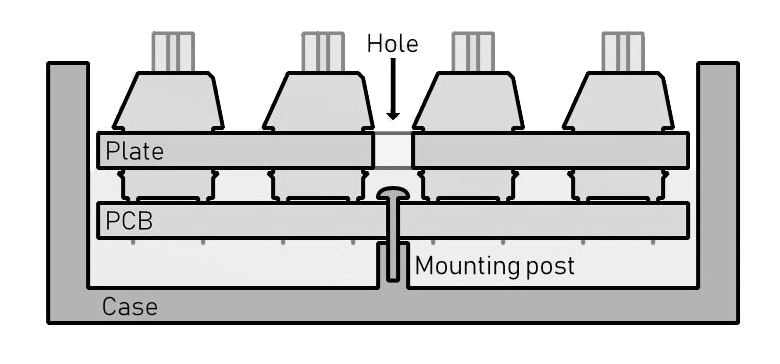
\includegraphics[width=0.73\textwidth]{imagenes/Capitulos/Cap03/Montajes/Montaje1.png}
        \caption{Montaje en carcasa inferior \cite{Keyboards-Mounting-Styles}}
        \label{fig:Montaje1}
    \end{figure}
    
    \item \textbf{Montaje en carcasa superior}: Atornillada a la parte superior de la carcasa que luego se monta sobre la inferior. Véase  la figura \ref{fig:Montaje2}.
    \begin{figure}[H]
        \centering
        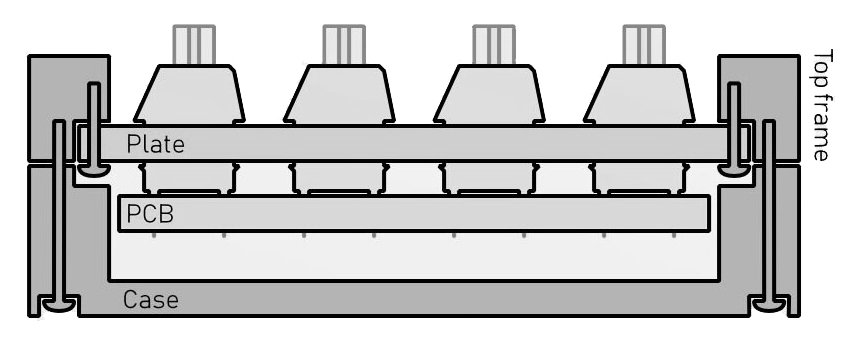
\includegraphics[width=0.7\textwidth]{imagenes/Capitulos/Cap03/Montajes/Montaje2.png}
        \caption{Montaje en carcasa superior \cite{Keyboards-Mounting-Styles}}
        \label{fig:Montaje2}
    \end{figure}
    
    \item \textbf{Montaje en carcasa inferior escondida}: Atornillada a la carcasa inferior. Véase  la figura \ref{fig:Montaje3}.
    \begin{figure}[H]
        \centering
        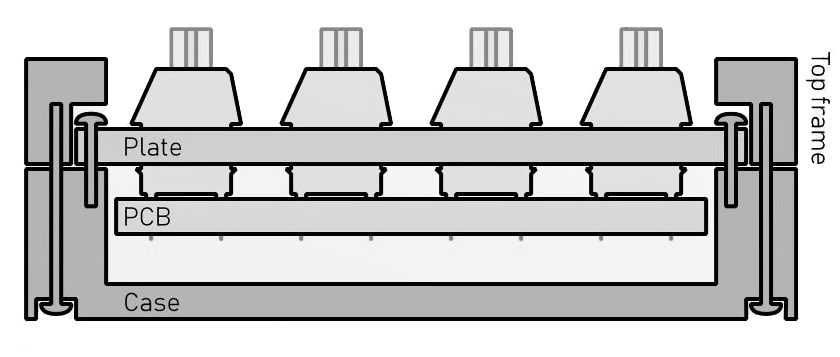
\includegraphics[width=0.7\textwidth]{imagenes/Capitulos/Cap03/Montajes/Montaje3.png}
        \caption{Montaje en carcasa \cite{Keyboards-Mounting-Styles}}
        \label{fig:Montaje3}
    \end{figure}
    
    \item \textbf{Montaje en carcasa sandwich}: Atornillada siendo atravesada por la carcasa inferior desde la parte de abajo hasta la carcasa superior. Véase  la figura \ref{fig:Montaje4}.
    \begin{figure}[H]
        \centering
        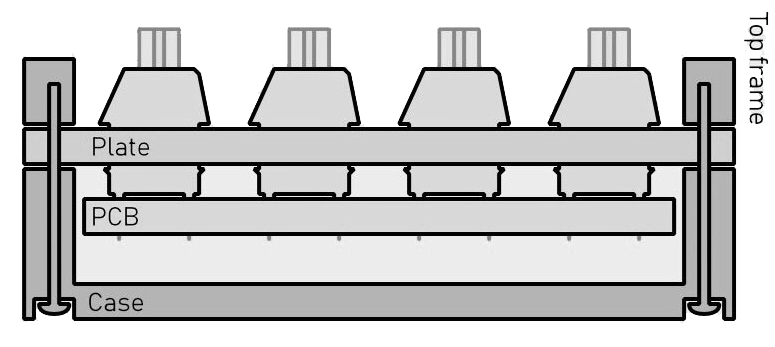
\includegraphics[width=0.7\textwidth]{imagenes/Capitulos/Cap03/Montajes/Montaje4.png}
        \caption{Montaje en carcasa sandwich \cite{Keyboards-Mounting-Styles}}
        \label{fig:Montaje4}
    \end{figure}
    
    \item \textbf{\gls{Plate} como carcasa superior}: La \glsnocase{Plate} toma el rol de ser también la tapa o carcasa del teclado. Véase  la figura \ref{fig:Montaje5}.
    \begin{figure}[H]
        \centering
        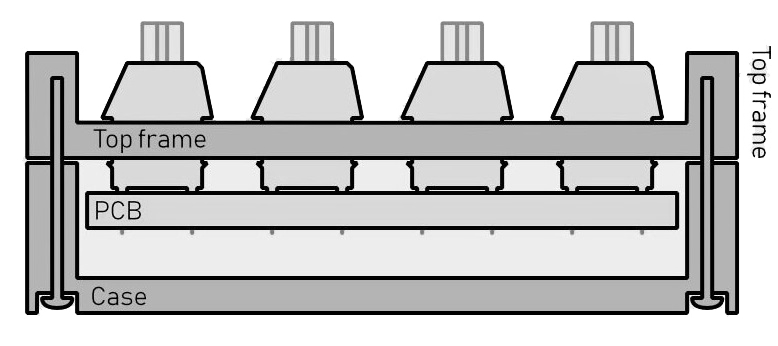
\includegraphics[width=0.7\textwidth]{imagenes/Capitulos/Cap03/Montajes/Montaje5.png}
        \caption{Montaje en forma de carcasa superior \cite{Keyboards-Mounting-Styles}}
        \label{fig:Montaje5}
    \end{figure}
    
    \item \textbf{Montaje en empaquetado}: Al igual que el sandwich solo que esta queda bloqueada por unos pasadores además de ser atornillada. Véase  la figura \ref{fig:Montaje6}.
    \begin{figure}[H]
        \centering
        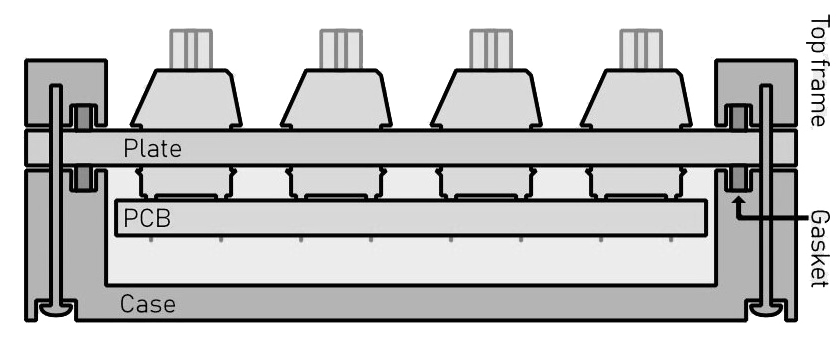
\includegraphics[width=0.7\textwidth]{imagenes/Capitulos/Cap03/Montajes/Montaje6.png}
        \caption{Montaje en empaquetado \cite{Keyboards-Mounting-Styles}}
        \label{fig:Montaje6}
    \end{figure}
    
    \item \textbf{Montaje sin \glsnocase{Plate}}: Este modo no usa \glsnocase{Plate} a la hora de construir el teclado. Véase  la figura \ref{fig:Montaje7}.
    \begin{figure}[H]
        \centering
        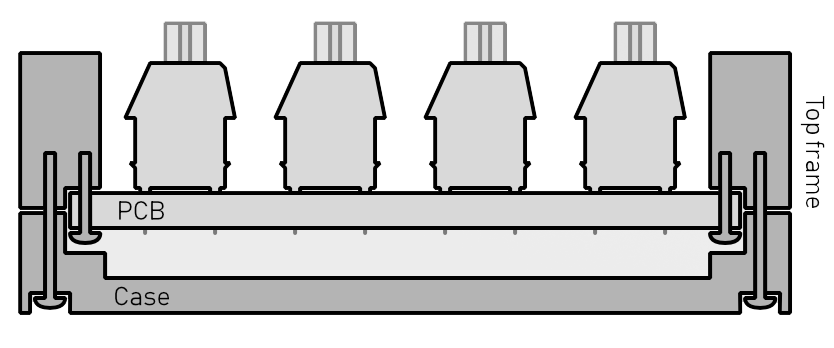
\includegraphics[width=0.7\textwidth]{imagenes/Capitulos/Cap03/Montajes/Montaje7.png}
        \caption{Montaje sin \glsnocase{Plate} \cite{Keyboards-Mounting-Styles}}
        \label{fig:Montaje7}
    \end{figure}
    
\end{itemize}
\newpage
La opción sin \glsnocase{Plate}, figura \ref{fig:Montaje7}, es la opción que se ha escogido para nuestro teclado. Ya que facilitara el diseño, abaratara el presupuesto y simplificara el montaje.

Para hacernos una idea está sería una \glsnocase{Plate} convencional de un teclado 60\% son sus tornillos correspondientes, tenemos la figura \ref{fig:Plate} con la que podemos hacernos una idea de cómo sería una \glsnocase{Plate} de un teclado convencional.

\begin{figure}[H]
    \centering
    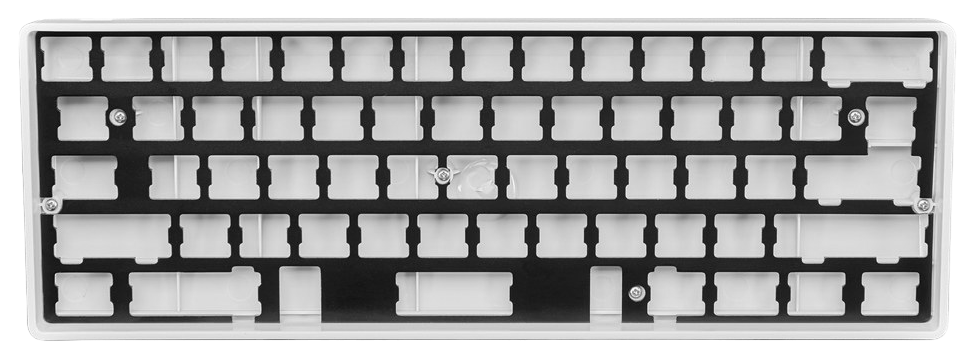
\includegraphics[width=1\textwidth]{imagenes/Capitulos/Cap03/Plate.png}
    \caption{Plate \cite{PlateImageSource}}
    \label{fig:Plate}
\end{figure}

\subsubsection{\gls{PCB}}

La \gls{PCB}, o Placa de Circuito Impreso, es una parte fundamental de un teclado mecánico. Es una placa de material aislante, generalmente fibra de vidrio o resina epoxi, sobre la cual están montados los \glsnocase{Switches} y otros componentes electrónicos del teclado. La \gls{PCB} proporciona la estructura física para el ensamblaje de los componentes del teclado y permite la conexión eléctrica entre ellos.

Los circuitos impresos en la \gls{PCB} dirigen las señales eléctricas de las teclas presionadas a través de los \glsnocase{Switches} hacia el controlador del teclado, que luego las envía al dispositivo al que está conectado el teclado, como una computadora o una consola de juegos. Además, la \gls{PCB} puede contener componentes adicionales, como diodos para la función anti-fantasma y \gls{LED}s para la retroiluminación.

La calidad y el diseño de la \gls{PCB} pueden afectar la durabilidad, la capacidad de personalización y la eficiencia energética del teclado. En teclados personalizados, la \gls{PCB} a menudo es una parte importante del diseño y puede ser programable para permitir la personalización de las funciones de las teclas.

\subsubsection{Espuma}

La espuma de amortiguación de sonido es un componente opcional que se puede agregar a un teclado mecánico para reducir el ruido producido por las pulsaciones de las teclas. Esta espuma se coloca generalmente entre la placa \gls{PCB} y la carcasa inferior del teclado, ayudando a absorber las vibraciones y el ruido generado por las pulsaciones de las teclas.

Aunque la espuma de amortiguación de sonido puede mejorar la experiencia auditiva al usar el teclado, su inclusión es opcional y depende de las preferencias personales del usuario. Algunas personas prefieren el sonido más nítido y distintivo de un teclado sin espuma de amortiguación, mientras que otras prefieren un teclado más silencioso y amortiguado.

La calidad y el tipo de espuma utilizada pueden afectar la eficacia de la amortiguación de sonido. Algunos teclados personalizados vienen con espumas específicamente diseñadas para reducir el ruido, mientras que otros pueden permitir que los usuarios añadan su propia espuma según sus necesidades y preferencias.

\subsubsection{Carcasa Inferior}

La carcasa inferior de un teclado es la parte que cubre la parte inferior del teclado y proporciona soporte estructural. Esta carcasa puede estar hecha de plástico u otros materiales resistentes y generalmente contiene la placa \gls{PCB} y otros componentes internos del teclado. Esta Proporciona una base sólida para los componentes internos y ayuda a protegerlos de daños externos. Si vemos la figura \ref{fig:BottomCase} podemos hacernos una idea de cómo sería una carcasa inferior de un teclado 60\% realizada en metal.

La carcasa inferior puede tener características adicionales, como patas ajustables para elevar la inclinación del teclado, o canales de enrutamiento para cables, que mejoran la comodidad y la organización al usar el teclado.

\begin{figure}[H]
    \centering
    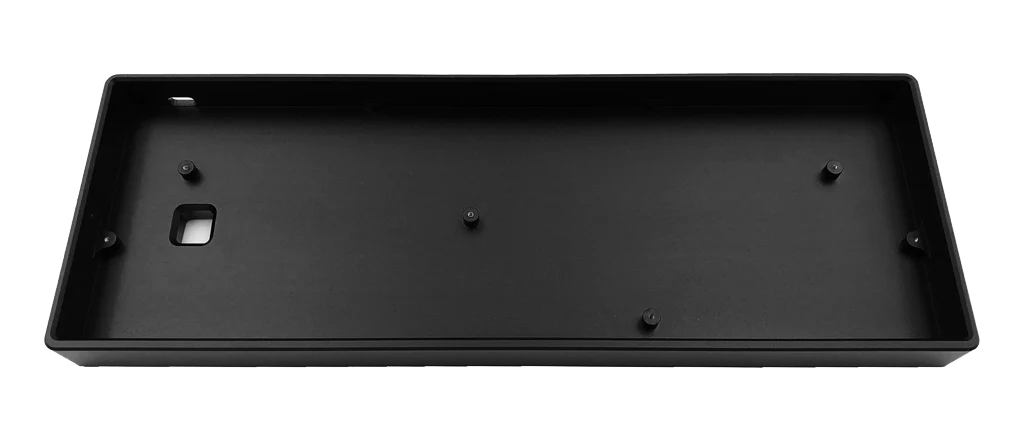
\includegraphics[width=0.7\textwidth]{imagenes/Capitulos/Cap03/BottomCase.png}
    \caption{Carcasa Inferior de Metal de teclado 60\%}
    \label{fig:BottomCase}
\end{figure}

\section{Investigación: Herramientas y Tecnologías}

La investigación y elección de herramientas y tecnologías son elementos fundamentales en el desarrollo de cualquier proyecto. En esta etapa, nos centraremos en identificar y evaluar diversas opciones disponibles en el panorama tecnológico actual, prestando especial atención a criterios clave como accesibilidad, robustez, comunidad de soporte y facilidad de integración. Abordaremos las necesidades específicas de cada fase del proyecto, desde el desarrollo de hardware hasta el software, con el objetivo de seleccionar herramientas y tecnologías que maximicen la eficiencia y la sinergia entre los componentes del sistema.

Aunque a lo largo de esta etapa se han llegado a encontrar alternativas mejores, estas supondrían un coste/beneficio demasiado alto para su desarrollo en el cuadro de tiempo dado.
Ya que estas suponen una curva de aprendizaje o coste de compra/uso demasiado alto para ser abordables. Aunque estas se mencionaran en cada sección y aparecerán descartadas por falta de tiempo o recursos. Aun así para alguien con el tiempo suficiente y la preparación necesaria serían sin duda la mejor elección.

En todas las secciones próximas se expondrán las elecciones realizadas en cada ámbito. Y también se expondrán todas y cada una de las alternativas que se hayan llegado a considerar junto a la explicación de porque han sido descartadas. Finalmente, se mostrará una tabla con los pros y contras para que cada uno pueda tomar sus decisiones a cerca de estas elecciones.

\section{Alternativas de diseño}
Aquí vamos a contemplar las diferentes opciones que tenemos a la hora de hacer un teclado, ya que como se ha mencionado antes, hay muchos formatos y tipos de teclados. Directamente y personalmente sé cuál va a ser el diseño elegido, ya que ando buscando un tipo de teclado que no he podido llegar a encontrar en decenas de páginas \glsnocase{Online} que he visitado y que cumplen las características siguientes:
\begin{itemize}
\item \gls{ISO} \\ La distribución será la \gls{ISO}, ya que mi idioma principal es el castellano.
\item 100\% o 105 \\ El teclado quiero que tenga todas las teclas que puede tener un teclado convencional, incluyendo el teclado numérico y teclas de función. En este caso, al ser \gls{ISO} la cantidad de teclas para llegar al 100\% son 105.
\item \gls{Bluetooth} \\ Conectividad inalámbrica.
\item Conectividad por cable \\ Para poder usar el teclado en un modo de baja \glsnocase{Latencia}.
\item Interruptores Mecánicos. \\ Para asegurar todo tipo de sensaciones a la hora de escribir. En mi caso Interruptores lineales.
\end{itemize}

\subsection{Elección de las herramientas} \label{Herramientas}
Vamos a empezar por las herramientas de diseño, la primera de todas la que hemos usado para crear los esquemas y planos del teclado, tomar medidas y planificar todo el diseño.

\begin{itemize}    
    \item Planos \\
    Las herramientas que se han encontrado para la creación de los planos son básicamente dos, una de pago y otra opción de software libre. Estas son AutoCAD y QCad. Dado que poseo una licencia de AutoCAD y personalmente tengo experiencia en esta herramienta he decidido usar esta herramienta para la creación de los planos del teclado. Para así poder ubicar todos los elementos de forma sencilla y sus dimensiones.
    
    \item Diseño de \gls{PCB} \\
    Existen varias opciones disponibles en el mercado para el diseño de \gls{PCB}. Algunas de las más populares son Altium Designer, KiCad, Eagle. Todos ellos son bastante parecidos en cuanto a las funcionalidades que se van a usar para el proyecto. Como se ha mencionado con las herramientas para los planos, también tenemos de pago y de software libre. Realmente aquí se ha escogido la herramienta por su conocimiento previo gracias a materias del grado como Diseño de Circuitos Impresos, donde se trabajó con Eagle. Por lo que el teclado está realizado con la herramienta Eagle.
    
    \item Editor de Texto/Programación \\
    Aquí disponemos de muchas opciones, entre las más famosas tenemos VSCode, Vim, \gls{Arduino} Editor (Si se usa \gls{Arduino}) o Sublime. Por conveniencia y uso a lo largo del tiempo, se va a usar VSCode, ya que se dispone del framework \gls{PlatformIO}, que es el que se va a usar a posteriori para programar nuestro controlador y diseñar el programa/\glsnocase{Firmware}.
    
    \item Software 3D \\
    Aquí tenemos las opciones más sencillas de diseño 3D, FreeCAD y Fusion360. Como ambas permiten las mismas opciones, se ha elegido FreeCAD como software de edición 3D.
    
    \item \gls{CNC} Corte \\
    En la búsqueda de software para crear los archivos necesarios para hacer funcionar la gls{CNC} para así hacer la carcasa se han encontrado diversos programas. Aunque la elección es clara, FreeCAD, ya que tenemos los archivos 3D ya en la aplicación y no tenemos que hacer nada más.
    
\end{itemize}
\newpage
%\subsubsection{Pros y Contras}

\section{Elección de Hardware} \label{DiseñoHardware}
En esta sección se van a tratar las diferentes opciones para los materiales. Los componentes electrónicos, las diferentes partes del teclado y el porqué de estas.

\subsection{Layout} \label{DiseñoLayaout}
Lo primero que se necesitó es conocer las dimensiones de la distribución. Así que buscando entre varias páginas encontré una herramienta que se llama ``Keyboard-Layout-Editor`` \cite{Layout-Editor} esta directamente te dejaba personalizar la distribución. La única modificación que sufrió la distribución \gls{ISO} fue que bajé las teclas especiales de la sección Print-Screen a al bloque de Pause/Delete. Esto fue pensado a futuro para poder colocar la electrónica en un sitio accesible. Esta modificación se puede ver en la figura \ref{fig:eISo_layout_modificado}, tenemos de referencia la distribución \gls{ISO} en la figura \ref{fig:ISO_layout} que sería la distribución original del teclado.

\begin{figure}[H] % Colocar las figuras exactamente aquí
    \centering
    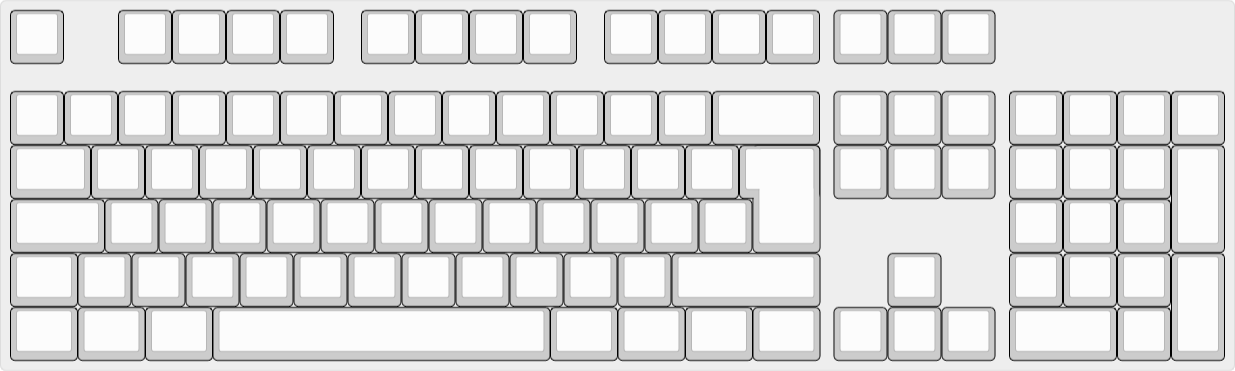
\includegraphics[width=1\textwidth]{imagenes/Capitulos/Cap03/ISO105Layout.png}
    \caption{\gls{ISO} 105 sin modificar}
    \label{fig:ISO_layout}
\end{figure}

\begin{figure}[H] % Colocar las figuras exactamente aquí
    \centering
    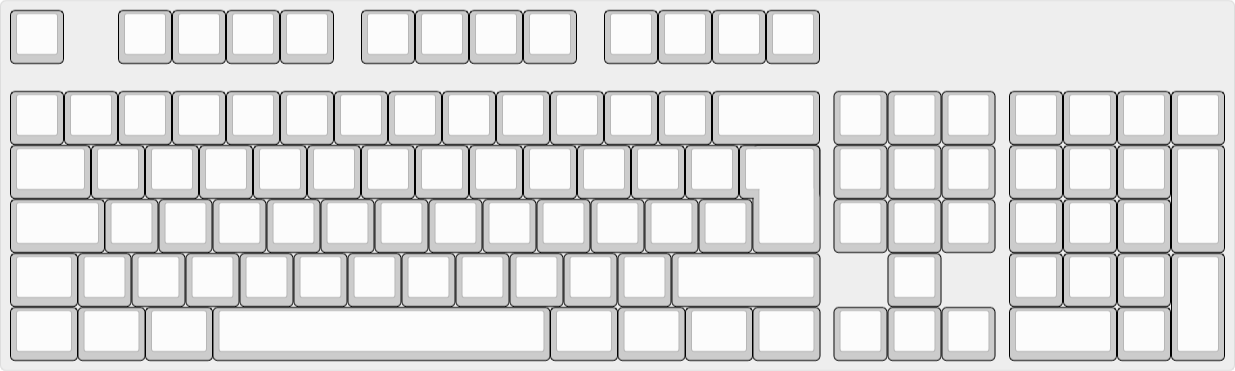
\includegraphics[width=1\textwidth]{imagenes/Capitulos/Cap03/ModernWoodLayout.png}
    \caption{\gls{ISO} 105 Modificado para el teclado ModernWood}
    \label{fig:eISo_layout_modificado}
\end{figure}

Esta herramienta permite exportar el esquema del teclado en un .JSON que posteriormente será necesario para usarlo en la página de ``Plate \& Case Builder`` \cite{builder-swillkb}. Esta herramienta no da un archivo .DWG que es un formato de AutoCAD para planos. El plano que nos ofrece es la plancha del teclado. Aunque nuestro teclado no va a utilizar, esta nos servirá posteriormente para diseñar la \gls{PCB} y la carcasa, ya que nos dirá donde va cada interruptor de forma muy precisa.

\subsection{Componentes Electrónicos}
A lo largo de toda la investigación he ido encontrando muchas alternativas para realizar el teclado, diferentes sistemas, diferentes microcontroladores y diferentes tipos de circuitos.

\subsubsection{Microcontrolador}
Este es el cerebro del teclado, este va a ser el encargado de la comunicación, de registrar las teclas, de construir los paquetes de datos, de mostrar los datos correspondientes y de mantener toda la iluminación.

Por esto es la pieza sobre lo que gira todo el proyecto y la parte más importante, también hay que considerar la facilidad para programarlos y la cantidad de recursos que tiene, tanto de librerías como de documentación.
Cuanto más extendido sea el uso, más sencillo será lograr que funcione.

A lo largo del periodo de investigación y diseño se han encontrado varias alternativas. Estas tienen que cumplir que tenga un hardware dedicado a la conectividad \gls{USB} llamado ``\gls{USB} OTG`` ya que se ideó así en la sección \ref{DiseñoConectividadCable}. Los principales y más destacables son:

\begin{itemize}
    \item \textbf{Atmega32u4}: Es un microcontrolador de la familia AVR de Atmel. Es ampliamente utilizado en proyectos de electrónica, especialmente en entornos \gls{Arduino}. Ofrece una buena cantidad de recursos y es fácil de programar.
    
    \item \textbf{STM32F103C8T6}: Es un microcontrolador de la familia STM32 de STMicroelectronics. Ofrece un buen equilibrio entre potencia de procesamiento y recursos. Es popular en proyectos de electrónica debido a su amplia disponibilidad y comunidad activa de usuarios.
    
    \item \textbf{nrf52840}: Es un microcontrolador de Nordic Semiconductor, diseñado específicamente para aplicaciones de conectividad inalámbrica de baja energía. Ofrece capacidades avanzadas de \gls{Bluetooth} y un bajo consumo de energía, lo que lo hace adecuado para dispositivos portátiles y \glsnocase{Wearable}s.
    
    \item \textbf{ESP32S3}: Es un microcontrolador de Espressif Systems, conocido por su conectividad \gls{WiFi} y \gls{Bluetooth} integrada. Ofrece una potencia de procesamiento considerable y una amplia gama de recursos.
\end{itemize}
Cada uno de estos microcontroladores ofrece pros y contras al proyecto.
\newpage
\subsubsection{Atmega32u4}
\begin{table}[H]
\centering
\small
\begin{tabular}{|p{0.45\linewidth}|p{0.45\linewidth}|}
\hline
\textbf{Pros} &
\textbf{Contras} \\
\hline
\parbox[t]{\linewidth}{
\vspace{0.1cm}
- Ampliamente utilizado y documentado en proyectos de teclado y dispositivos de entrada. \medskip \\
- Facilidad de programación con el ecosistema \gls{Arduino}. \medskip \\
- Integración de puertos \gls{USB} nativos, lo que facilita la comunicación. \medskip \\
- Fácil de soldar \medskip \\
- Librerías para \gls{PCB} \medskip \\
- Muy barato \medskip \\
- 5V \\
\vspace{0.1cm}
} &
\parbox[t]{\linewidth}{
\vspace{0.1cm}
- Requiere hardware adicional y configuración personalizada para habilitar la conectividad \gls{Bluetooth}. \medskip \\
- Limitaciones en términos de potencia de procesamiento y recursos en comparación con otros microcontroladores más orientados a la conectividad.} \medskip \\
\hline
\end{tabular}
\caption{Ventajas y desventajas de Atmega32u4}
\end{table}

\subsubsection{STM32F103C8T6}
\begin{table}[H]
\centering
\small
\begin{tabular}{|p{0.45\linewidth}|p{0.45\linewidth}|}
\hline
\textbf{Pros} &
\textbf{Contras} \\
\hline
\parbox[t]{\linewidth}{
\vspace{0.1cm}
- Soporte para una amplia variedad de librerías y documentación, incluidas las relacionadas con \gls{Bluetooth}. \medskip \\
- Potente y versátil, lo que facilita la implementación de soluciones \gls{Bluetooth} personalizadas. \medskip \\
- Ampliamente utilizado en aplicaciones de \gls{IoT} y sistemas embebidos, lo que puede ofrecer soluciones ya probadas para la conectividad \gls{Bluetooth}. \medskip \\
- Librerías para \gls{PCB} \medskip \\
- Fácil de soldar \medskip \\
- Barato
} &
\parbox[t]{\linewidth}{
\vspace{0.1cm}
- Requiere herramientas de desarrollo específicas y conocimientos más avanzados en programación. \medskip \\
- Curva de aprendizaje más pronunciada debido a su complejidad en comparación con los microcontroladores basados en \gls{Arduino}. \medskip \\
- Posiblemente excesivamente difícil para aplicaciones simples de teclado. \medskip \\
- Requiere hardware adicional y configuración personalizada para habilitar la conectividad \gls{Bluetooth}. \medskip \\
- Requiere el uso de su framework específico  \medskip \\
- 3.3V} \medskip \\
\hline
\end{tabular}
\caption{Ventajas y desventajas de STM32F103C8T6}
\end{table}

\subsubsection{Nrf52840}
\begin{table}[H]
\centering
\small
\begin{tabular}{|p{0.45\linewidth}|p{0.45\linewidth}|}
\hline
\textbf{Pros} &
\textbf{Contras} \\
\hline
\parbox[t]{\linewidth}{
\vspace{0.1cm}
- Diseñado específicamente para aplicaciones de baja potencia y conectividad inalámbrica, lo que lo hace ideal para la implementación de \gls{Bluetooth} de baja energía. \medskip \\
- Amplia gama de características de conectividad, incluido \gls{Bluetooth} de baja energía. \medskip \\
- Buen soporte de documentación y comunidad de desarrollo. \medskip \\
- Modo \glsnocase{Deep Sleep} para ahorrar energía
} &
\parbox[t]{\linewidth}{
\vspace{0.1cm}
- Sin librerías para \gls{PCB} Eagle \medskip \\
- Muy dificil de soldar \medskip \\
- Menos común en aplicaciones de teclado en comparación con otros microcontroladores. \medskip \\
- Requiere más experiencia en el desarrollo de sistemas inalámbricos y \gls{Bluetooth}. \medskip \\
- Requiere el uso de su framework específico. \medskip \\
- Caro. \medskip \\
- 3.3V} \medskip \\
\hline
\end{tabular}
\caption{Ventajas y desventajas de Nrf52840}
\end{table}

\subsubsection{ESP32S3}
\begin{table}[H]
\centering
\small
\begin{tabular}{|p{0.45\linewidth}|p{0.45\linewidth}|}
\hline
\textbf{Pros} &
\textbf{Contras} \\
\hline
\parbox[t]{\linewidth}{
\vspace{0.1cm}
- Capacidades de conectividad \gls{WiFi} y \gls{Bluetooth} integradas, lo que facilita la implementación de soluciones \gls{Bluetooth}. \medskip \\
- Potente y versátil, con una amplia comunidad de desarrollo y soporte de documentación. \medskip \\
- Ideal para proyectos que requieren conectividad inalámbrica y capacidades avanzadas de procesamiento. \medskip \\
- Con todo tipo de librerías \medskip \\
- Modo \glsnocase{Deep Sleep} para ahorrar energía \medskip \\
- Muy barato \vspace{0.3cm}
} &
\parbox[t]{\linewidth}{
\vspace{0.1cm}
- Dificultad media para soldar. \medskip \\
- Consumo alto de energía sin \glsnocase{Deep Sleep}. \medskip \\
- 3.3V } \medskip \\
\hline
\end{tabular}
\caption{Ventajas y desventajas de ESP32S3}
\end{table}

La elección final se va a volver a hacer en cuanto a estética y funcionalidad. Como buscar nuevo hardware para la conectividad \glsnocase{Bluetooth} iba a ser otra tarea costosa en cuanto a tiempo y recursos, los microcontroladores que necesitasen un hardware específico para la conectividad han sido descartados.
Lo que nos deja solo con ESP32S3 y Nrf52840. Entre estos dos, dada la dificultad de aprendizaje, la dificultad muy alta para soldarlo a la \gls{PCB} y que hay menos documentación, nos vamos a quedar con el microcontrolador \textbf{ESP32S3}. Una vez que ya sabemos qué microcontrolador vamos a usar podemos atender a las diferentes secciones.

\subsubsection{Sistema de Batería} \label{InvestigacionSistemaBateria}
Como se ideó en la sección de diseño \ref{DiseñoBateriaAlimentacion} y dado que el hueco para albergar la batería es pequeño y bastante plano, ya que tiene que ir entre la placa \gls{PCB} y la carcasa no hay muchas opciones. Esta será una batería Li-ion (Ion Litio) y dado que el microcontrolador funciona a 3.3V tendremos que buscar una batería típica de 3.7V.

Ahora el problema subyacente es cargar la batería y al mismo tiempo poder usar el teclado sin que esta se dañe. Buscando alternativas y modos de realizar esta tarea se ha encontrado un módulo para desarrollo llamado TP4056 que contiene un sistema de protección de la batería y un sistema de carga y consumo en paralelo manteniendo la vida de la batería, podemos ver este circuito en la figura \ref{fig:SchemeTP4056}. Como se quiere aun así mantener la estética, no se empleara el módulo directamente, sino que se buscara un esquemático del módulo y se implementará directamente sobre la \gls{PCB}. Se han encontrado varios archivos esquemáticos.

\begin{figure}[H]
    \centering
    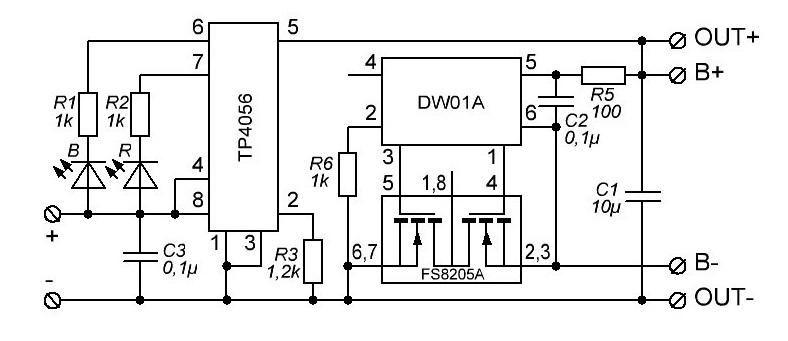
\includegraphics[width=1\textwidth]{imagenes/Capitulos/Cap03/TP4056Schematic.png}
    \caption{Esquemático del modulo TP4056 \cite{TP4056SchematicInternet}}
    \label{fig:SchemeTP4056}
\end{figure}

\subsubsection{Sistema de Pantalla} \label{DiseñoPantalla}
La idea es que este teclado dispusiera de una pantalla para mostrar información básica del estado del teclado, configuración y un menú de usuario. La búsqueda de una pantalla tampoco ha supuesto un gran reto. Solo tenía que cumplir varios requisitos. Que cupiese en el área designada para la electrónica y que fuera compatible con el microcontrolador. Hay dos pantallas que cupiesen en el área designada y no fueran unan \gls{LCD} de poca resolución, estas son la \textbf{\gls{TFT} 0.96"} y la \textbf{\gls{OLED} 0.96"}. Entre estas dos se tenía que escoger una.

\subsubsection{\gls{TFT} 0.96"}
\begin{table}[H]
\centering
\small
\begin{tabular}{|p{0.45\linewidth}|p{0.45\linewidth}|}
\hline
\textbf{Pros} &
\textbf{Contras} \\
\hline
\parbox[t]{\linewidth}{
\vspace{0.1cm}
- Pantalla a color que permite una representación más detallada. \medskip \\
- Fácil de programar y utilizar con librerías disponibles. \medskip \\
- Ideal para proyectos que requieren interfaces de usuario simples. \medskip \\
- Amplia disponibilidad y variedad de opciones en el mercado. \vspace{0.1cm}
} &
\parbox[t]{\linewidth}{
\vspace{0.1cm}
- Consumo moderado de energía, pero más alto que las pantallas \gls{OLED}. \medskip \\
\vspace{0.1cm}
} \\
\hline
\end{tabular}
\caption{Ventajas y desventajas de la pantalla TFT 0.96``}
\end{table}

\subsubsection{OLED 0.96"}
\begin{table}[H]
\centering
\small
\begin{tabular}{|p{0.45\linewidth}|p{0.45\linewidth}|}
\hline
\textbf{Pros} &
\textbf{Contras} \\
\hline
\parbox[t]{\linewidth}{
\vspace{0.1cm}
- Pantalla que ofrece un contraste superior a un solo color. \medskip \\
- Consumo de energía muy bajo, especialmente al mostrar contenido estático. \medskip \\
- Ángulos de visión más amplios y mejor visibilidad en condiciones de luz ambiental variable. \medskip \\
- Ideal para aplicaciones de bajo consumo. \medskip \\
\vspace{0.1cm}
} &
\parbox[t]{\linewidth}{
\vspace{0.1cm}
- Solo un color. \vspace{0.1cm}
} \\
\hline
\end{tabular}
\caption{Ventajas y desventajas de la pantalla OLED 0.96``}
\end{table}

Se ha acabado escogiendo la pantalla \textbf{\gls{TFT} 0.96"} solo por la cantidad de colores que puede mostrar. Esta usa 8 pines de nuestro microcontrolador.

\subsubsection{Sistema de \glsnocase{Polling}}
Dado que los microcontroladores no tienen la cantidad de pines necesarios para conectar la matriz de pines de 16x6 en total son necesario 22 pines exclusivamente para todas las teclas. Recordando materias de electrónica, recordé la existencia de un dispositivo que permite multiplexar señales eléctricas. Dado que tenemos que ir recorriendo las secciones verticales una a una e ir leyendo las horizontales para saber qué tecla se ha pulsado, podemos multiplexar esas 16 líneas en tan solo 4 gracias al dispositivo \glsnocase{Multiplexor}. Para hacernos una idea de como es la matriz de teclado podemos ver la figura \ref{fig:EjemploArrayTeclado}.

El objetivo es encontrar un \glsnocase{Multiplexor} que quepa y que nos ofrezca la función de 4 a 16, que valga a 3.3V y que pueda ser soldado con facilidad. Tan solo con una búsqueda aparece el \textbf{CD74HC154M96} dado que directamente cumple todos los requisitos pedidos nos vamos a quedar con este.

Esto nos permitirá configurar el microcontrolador con 4 pines de salida para seleccionar la columna que queremos comprobar y leer los 6 pines configurados como entrada para saber qué tecla exacta está o no pulsada.

\begin{figure}[H]
    \centering
    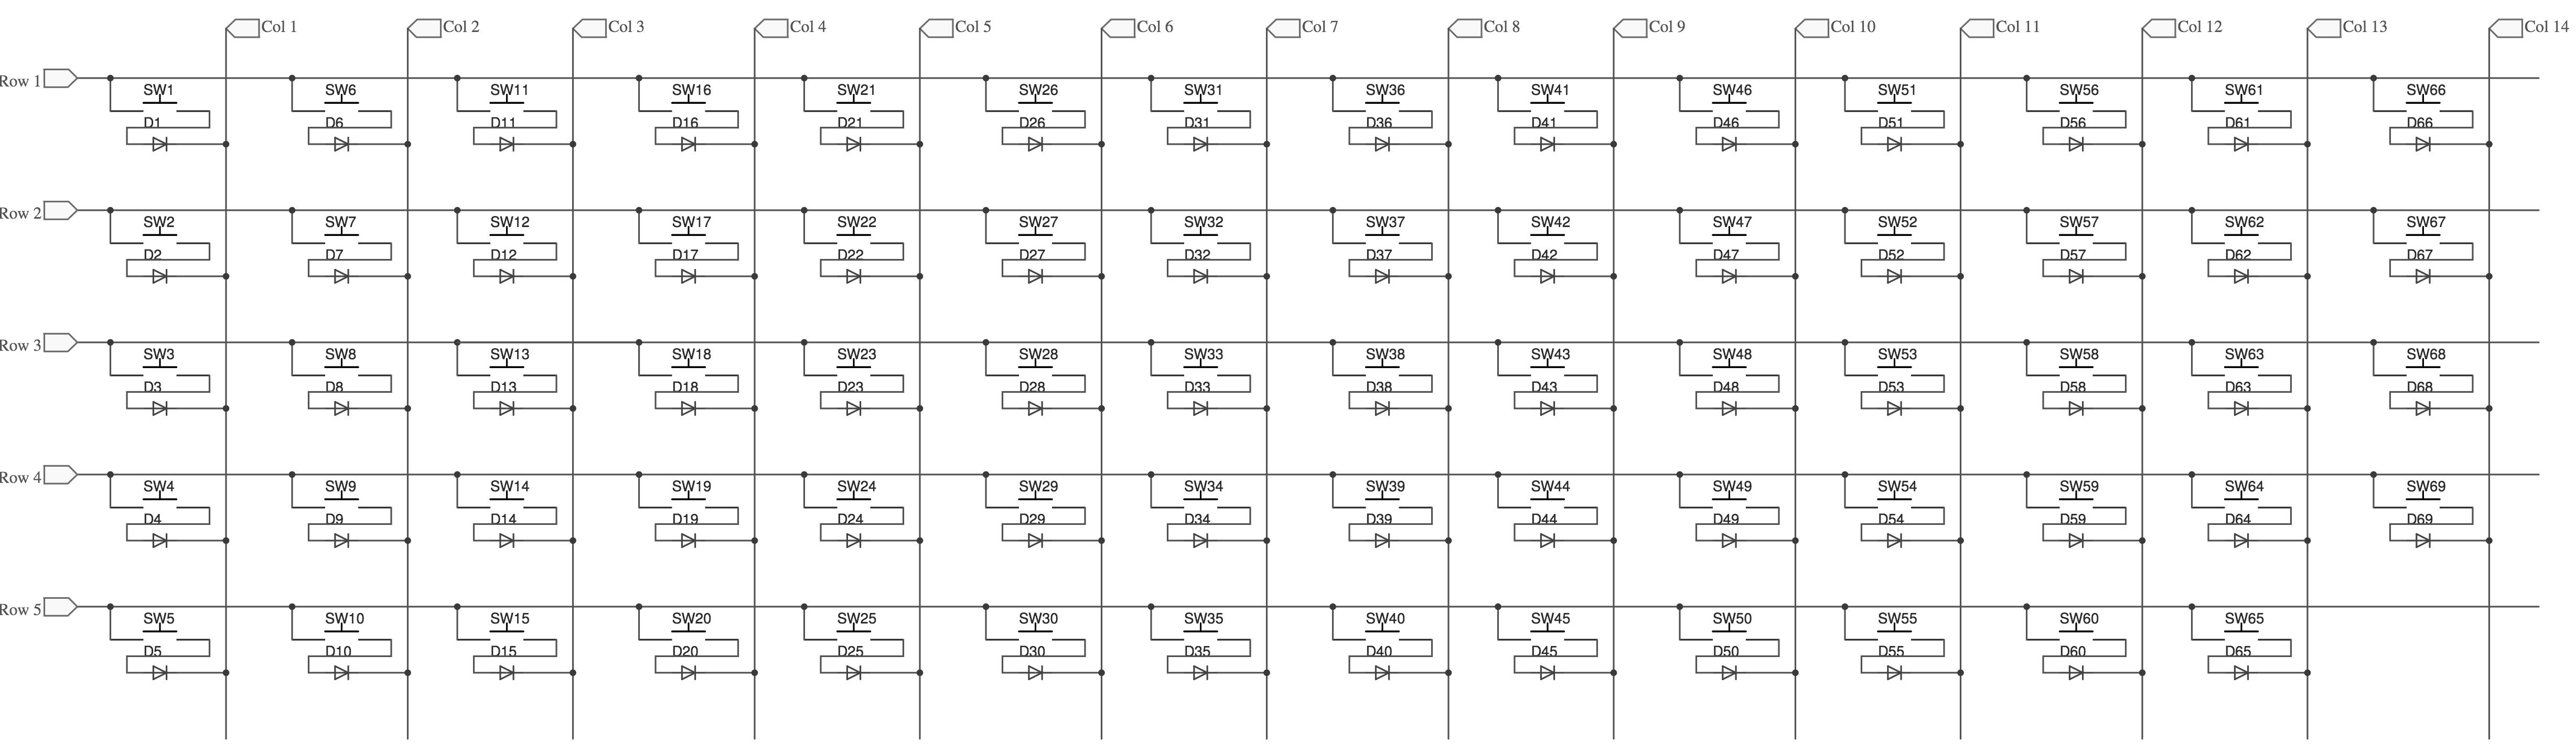
\includegraphics[width=1\textwidth]{imagenes/Capitulos/Cap03/EjemploArrayTeclado.png}
    \caption{Ejemplo básico de matriz de teclado \cite{EjemploArrayTeclado}}
    \label{fig:EjemploArrayTeclado}
\end{figure}

\newpage
\subsubsection{Conexión \gls{USB}} \label{DiseñoConexiones}
Como estamos usando un microcontrolador que dispone de \gls{USB}-OTG no será necesario usar un elemento hardware externo que nos permita comunicarnos con el protocolo \gls{USB}. Este ya vendrá por defecto en el ESP32S3.

Eso sí, necesitaremos mirar qué pines están conectados al módulo de \gls{USB} en el ESP32S3. Para la conexión al exterior usaremos simplemente un cable conectando la \gls{PCB} al conector de aviación XS-12 que nos asegure la robustez que se ideó en la sección \ref{RequisitosNoFuncionales}. El conector XS-12 se puede ver abajo en la figura \ref{fig:XS12}.

\begin{figure}[H]
    \centering
    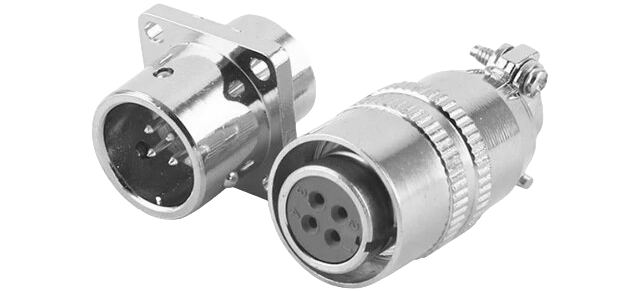
\includegraphics[width=0.75\textwidth]{imagenes/Capitulos/Cap03/XS12.png}
    \caption{Imagen del conector XS-12}
    \label{fig:XS12}
\end{figure}

Este conector irá atornillando a la carcasa y luego se fabricara un cable de este conector a \gls{USB} tipo A. usando un cable reforzado de 4 hilos internos y dos conectores más. Un conector de seguridad GX16 de 4 pines para darle robustez y un acabado más estético y un cabezal \gls{USB} A chapado en oro y todo sellado con tubo \glsnocase{Termoretractil}. El conector GX16 podemos verlo en la figura \ref{fig:GX16} y asi hacernos una idea de cómo será el conector \gls{USB} y el tipo A en la figura \ref{fig:USBA}.

\begin{figure}[H]
    \centering
    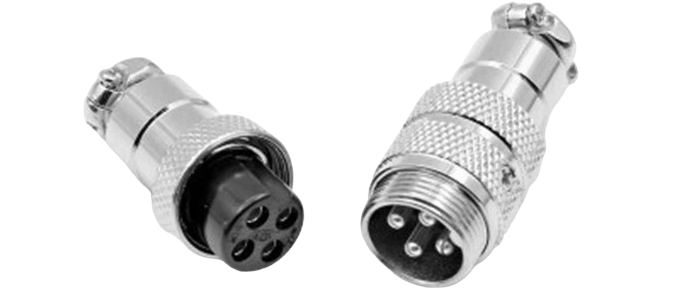
\includegraphics[width=0.8\textwidth]{imagenes/Capitulos/Cap03/GX16.png}
    \caption{Imagen del conector GX-16}
    \label{fig:GX16}
\end{figure}

\begin{figure}[H]
    \centering
    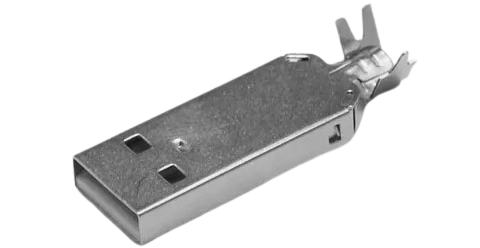
\includegraphics[width=1\textwidth]{imagenes/Capitulos/Cap03/USBA.png}
    \caption{Imagen del conector \gls{USB} tipo A}
    \label{fig:USBA}
\end{figure}


\subsubsection{Sistema de \gls{LED}S} \label{DiseñoLeds}
Se han elegido los \gls{LED}S programables que se usan en las tiras comunes, ya que permiten muchas combinaciones y son muy baratos y sencillos de programar, además de que solo usan un pin del microcontrolador. La elección más sencilla ha sido para \textbf{WS2812B-B/W} que es el modelo más común y más barato. Podemos ver una imagen de este \gls{LED} en la figura \ref{fig:WS2812B}.

\begin{figure}[H]
    \centering
    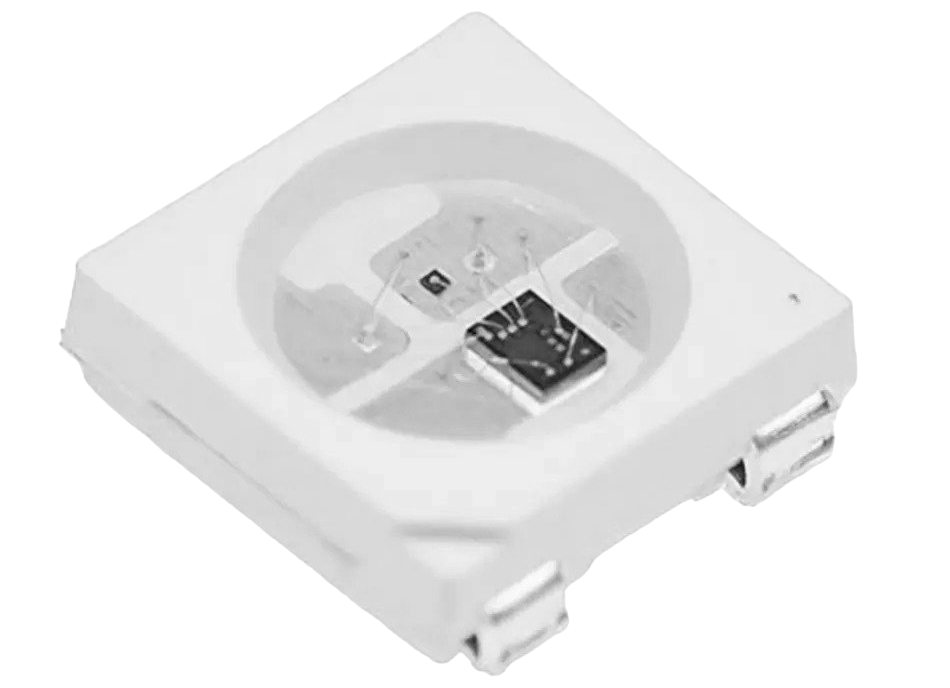
\includegraphics[width=0.8\textwidth]{imagenes/Capitulos/Cap03/WS2812B.png}
    \caption{Imagen del \gls{LED} WS2812B}
    \label{fig:WS2812B}
\end{figure}

\subsection{Materiales}
Desde un principio la elección clara era madera, ya que se quería conseguir una estética natural y tecnológica juntas. Las maderas serán a elección del usuario, para que pueda escoger tanto color, tipo de veta y sensación al tacto.
Por lo tanto esta subsección se tratara de gustos personales. Entre las elecciones para este proyecto se han considerado \textbf{Jatoba, Sucupira y Mansonia}, además se añadirán detalles en metacrilato o acrílico para proteger los componentes que son visibles, ya que el teclado esta diseñado para ser un teclado sin \glsnocase{Plate}.

\subsection{Partes del teclado}
Durante la fase de diseño \ref{DiseñoDistribucion} se han hecho elecciones de como va a ser el teclado, y de qué cosas dispondrá este. En esta subsección se hará un breve resumen. El teclado se compondrá de una carcasa en forma de cajón donde la \gls{PCB} irá atornillada y no tendrá \glsnocase{Plate}. Los interruptores se colocarán soldados sobre la \gls{PCB} con las \glsnocase{Keycaps}. De forma adicional se colocarán unas placas de acrílico sobre los componentes electrónicos para protegerlos y que aun así queden vistos. La tornillería se compondrá de elementos como separadores y de tornillos M3 negros.

La electrónica se compondrá de un ESP32S3 un \glsnocase{Multiplexor} para el mapeo de las teclas, una pantalla \gls{TFT} de 0.96", una batería, un circuito específico para la batería (TP4056) y todo el cableado \gls{USB}.
\newpage

\section{Elección de Software}
En esta sección se van a tratar las diferentes opciones para las elecciones que tenemos de herramientas para desarrollar el \glsnocase{Firmware} para el ESP32S3 y qué librerías se van a usar para ello.

\subsection{Entorno de desarrollo}
Dado que vamos a trabajar con un ESP32S3 tenemos múltiples opciones, \textbf{Arduino IDE}, \textbf{PlatformIO} y \textbf{Espressif ESP-IDF}.

Estas alternativas están ordenadas de menor a mayor complejidad y funcionalidad.
\subsubsection{Arduino IDE}
\gls{Arduino} IDE se compone un programa que permite la edición de un archivo .ino que posteriormente se compila y se sube al microcontrolador. Dado que es muy sencillo este entorno, está muy muy limitado para proyectos con varios archivos, librerías personalizadas y código C. Esta queda directamente descartada, ya que nuestro proyecto estará si o si dividido en varios archivos y será mucho más sencillo en las otras.

\subsubsection{\gls{PlatformIO}} \label{DiseñoPlatformIO}
\gls{PlatformIO} es un entorno de desarrollo que reúne las herramientas necesarias para el desarrollo de proyectos de hardware, especialmente en microcontroladores como Atmega, ESP32, STM32, entre otros. Ofrece una solución más avanzada y versátil en comparación con el \gls{Arduino} IDE.

Permite la creación y gestión de proyectos complejos que involucran múltiples archivos, bibliotecas personalizadas y configuraciones específicas para diferentes placas y microcontroladores.

Facilita la inclusión y gestión de bibliotecas externas a través de su sistema de gestión de librerías integrado. También ofrece herramientas avanzadas de compilación y depuración que facilitan el desarrollo y la corrección de errores en el código.

Admite una amplia gama de microcontroladores y placas, lo que permite a los desarrolladores trabajar con diferentes dispositivos sin restricciones. Entre ellas el microcontrolador ESP32S3.

Además, \gls{PlatformIO} se integra con entornos de desarrollo integrado (IDE) como Visual Studio Code, Atom y Eclipse, lo que proporciona a los desarrolladores una experiencia de desarrollo más completa y personalizable.

\subsubsection{Espressif ESP-IDF}
El Espressif \gls{IoT} Development Framework (ESP-IDF) es un conjunto de herramientas de desarrollo de software diseñado específicamente para trabajar con microcontroladores de la serie ESP32 de Espressif Systems. Este framework proporciona un entorno de desarrollo completo y robusto para la creación de aplicaciones y \glsnocase{Firmware} personalizado para dispositivos basados en ESP32.

El ESP-IDF está diseñado para aprovechar al máximo las capacidades y características del ESP32, incluyendo su procesador de doble núcleo, conectividad \gls{WiFi} y \glsnocase{Bluetooth}, y una amplia gama de periféricos integrados.

Viene con una amplia gama de bibliotecas y ejemplos de código que facilitan el desarrollo de aplicaciones para una variedad de propósitos, como la comunicación inalámbrica, la gestión de energía y la interfaz con sensores y actuadores.

Espressif proporciona una documentación exhaustiva y actualizada que cubre todos los aspectos del desarrollo con ESP-IDF, incluyendo guías de inicio rápido, tutoriales y referencias de \gls{API}.

En resumen, el Espressif ESP-IDF es un framework de desarrollo de software potente y versátil que ofrece a los desarrolladores todas las herramientas necesarias para crear aplicaciones personalizadas para dispositivos basados en ESP32, aprovechando al máximo las capacidades de estos microcontroladores. Pero dado que este es mucho más amplio, también es más complejo de usar.

\subsubsection{Elección final}

Dado todo lo anterior y que nuestro proyecto no va a requerir un código muy complejo y un control de muy bajo nivel sobre el microcontrolador, vamos a elegir \textbf{PlatformIO} que nos permitirá tener un proyecto grande compuesto de múltiples archivos y nos dará la suficiente libertad sin tener que invertir muchos recursos aprendiendo a usar ESP-IDF. Aun asi instalaremos ESP-IDF para compilar el código, ya que el compilador específico genera un mejor código.
\newpage
\subsection{Librerías} \label{DiseñoLibrerias}
En el apartado Hardware se han listado varios componentes que van a necesitar comunicarse con el Microcontrolador ESP32S3, entre ellos tenemos los \gls{LED}S, la pantalla \gls{TFT} 0.96". Pero también sera necesario activar y poder usar el \glsnocase{Bluetooth} como elemento \gls{HID}. Por lo que haciendo el recuento tenemos que buscar estas 3 librerías que nos permitan hacer uso de estos dispositivos.
\begin{itemize}
    \item \gls{LED}S\\
    Para los \glsnocase{LED}s con una simple búsqueda podemos encontrar que Adafruit (El fabricante de la pantalla) ya pone a disposición una librería compatible con nuestro Framework. Esta librería es la \textbf{Adafruit NeoPixel}.
    \item Pantalla \gls{TFT} 0.96"\\
    Al igual que para los \glsnocase{LED}s disponemos de una librería que nos permite hacer todo tipo de cosas con la pantalla, mostrar gráficos, imágenes y texto de forma sencilla. Esta está realizada por un particular en este caso. La librería se llama \textbf{TFT\_eSPI} \cite{TFTLib}.
    \item \gls{Bluetooth} \gls{HID}\\
    Aquí volvemos a encontrar que disponemos de una librería particular que nos resuelve el problema de mostrar nuestro teclado como un dispositivo \gls{HID} a otros dispositivos a través de \glsnocase{Bluetooth}, este también nos permite enviar caracteres al dispositivo conectado. Por lo que nos vendrá genial. La librería en este caso es la \textbf{NimBLE-Arduino} \cite{NimbleLib}.
\end{itemize}

\section{Presupuesto}
Esta sección presenta un listado detallado de los costos asociados al desarrollo y fabricación del producto. El presupuesto abarca diferentes aspectos del proyecto, desde la adquisición de materiales hasta los gastos relacionados con el personal y la investigación y desarrollo. También se proporcionará una lista de todos los componentes con su coste asociado y el precio de adquisición así como el lugar de donde se ha adquirido y el coste de envío. 
%En esta sección se tratara de forma breve el presupuesto, ya que se tratara de forma más extensa en la sección de comercialización \ref{SeccionCostosProduccion}.

\newpage
\subsubsection{Componentes Electrónicos}

En la tabla \ref{Table:ComponetesElectronicos} se puede ver el coste de todos estos componentes, estos han sido elegidos en base al precio, funcionalidad y tipo. 

El total de la suma de los componentes electrónicos supone: \textbf{67,76 \euro}

\begin{table}[!htb]
\small
\begin{tabular}{|l|l|l|l|r|}
\hline
Tipo                                                              & Elemento                                                                 & Cantidad & Proveedores & Precio \\ \hline
\gls{Multiplexor}                                                       & \begin{tabular}[c]{@{}l@{}}CD74HC154M96\\  (SOIC-24-300mil)\end{tabular} & 1 (5)    & lcsc.com    & 3.40    \\ \hline
Condensador                                                       & \begin{tabular}[c]{@{}l@{}}293D105X9035A2TE3 1uF \\ (1206)\end{tabular}  & 5 (20)   & lcsc.com    & 2.06   \\ \hline
Resistencia                                                       & \begin{tabular}[c]{@{}l@{}}RT0805BRD071KL 1k \\ (0805)\end{tabular}      & 5 (20)   & lcsc.com    & 0.68   \\ \hline
Resistencia                                                       & \begin{tabular}[c]{@{}l@{}}RC0805FR-071ML 1M \\ (0805)\end{tabular}      & 3 (100)  & lcsc.com    & 0.21   \\ \hline
Resistencia                                                       & \begin{tabular}[c]{@{}l@{}}0805W8F2004T5E 2M \\ (0805)\end{tabular}      & 2 (100)  & lcsc.com    & 0.16   \\ \hline
Resistencia                                                       & \begin{tabular}[c]{@{}l@{}}RC0805FR-073M74L 3.7M \\ (0805)\end{tabular}  & 1 (50)   & lcsc.com    & 0.18   \\ \hline
\begin{tabular}[c]{@{}l@{}}Circuito \\ Carga Batería\end{tabular} & \begin{tabular}[c]{@{}l@{}}TP4056 \\ (C725790)\end{tabular}              & 1 (5)    & lcsc.com    & 0.52   \\ \hline
\begin{tabular}[c]{@{}l@{}}C. Protección\\  Batería\end{tabular}   & \begin{tabular}[c]{@{}l@{}}DW01A \\ (SOT23-6)\end{tabular}               & 1 (20)   & lcsc.com    & 0.41   \\ \hline
\begin{tabular}[c]{@{}l@{}}C. Protección \\ Batería\end{tabular}   & \begin{tabular}[c]{@{}l@{}}ME6211C33M5G \\ (SOT-23-5)\end{tabular}       & 1 (10)   & lcsc.com    & 0.48   \\ \hline
\begin{tabular}[c]{@{}l@{}}C. Protección \\ Batería\end{tabular}   & \begin{tabular}[c]{@{}l@{}}FS8205A \\ (TSSOP-8)\end{tabular}             & 1 (10)   & lcsc.com    & 0.62   \\ \hline
Chip Principal                                                    & \begin{tabular}[c]{@{}l@{}}ESP32-S3 \\ (SMD,18x25.5mm)\end{tabular}      & 1 (1)    & lcsc.com    & 4.46   \\ \hline
Leds                                                              & \begin{tabular}[c]{@{}l@{}}WS2812B \\ (C114586)\end{tabular}             & 10 (25)  & lcsc.com    & 2.18   \\ \hline
Diodos                                                            & \begin{tabular}[c]{@{}l@{}}1N5819W \\ (SOD123FL)\end{tabular}            & 96 (250) & lcsc.com    & 2.08   \\ \hline
\gls{PCB}                                                               & \begin{tabular}[c]{@{}l@{}}Placa Base \gls{DIY} \end{tabular}            & 1 (5) & jlcpcb.com  & 42.76  \\ \hline
Envíos                                                            & \begin{tabular}[c]{@{}l@{}}Envio Piezas \end{tabular}                    & 1 (1) & lcsc.com    & 7.56   \\ \hline
\hline
\multicolumn{4}{|l|}{Total} & 67.76 \\
\hline
\end{tabular}
\caption{Componentes electrónicos}
\label{Table:ComponetesElectronicos}
\end{table}

\newpage
\subsubsection{Componentes de Montaje}

En la tabla \ref{Table:ComponentesMontaje} se puede ver el coste de todos estas piezas y partes, estos han sido elegidos en base al precio, estética y funcionalidad. 

El total de la suma de los componentes para montaje supone:  \textbf{185,83 \euro}

\begin{table}[!htb]
\small
\begin{tabular}{|l|l|l|l|r|}
\hline
Tipo                                                              & Elemento                                                                                       & Cantidad                                                                           & Proveedores & Precio \\ \hline
\begin{tabular}[c]{@{}l@{}}Partes\\ Cable\end{tabular}            & \begin{tabular}[c]{@{}l@{}}Paracord negro\\ de 9 núcleos\end{tabular}                          & 1 (1)                                                                              & \raggedleft \begin{tabular}[c]{@{}l@{}}Aliexpress\\ Qiuhike\end{tabular}    & 3.16   \\ \hline
\begin{tabular}[c]{@{}l@{}}Partes\\ Cable\end{tabular}            & \begin{tabular}[c]{@{}l@{}}Cabeza \gls{USB} A\\ Chapada en Oro\end{tabular}                          & 1 (5)                                                                              & \raggedleft \begin{tabular}[c]{@{}l@{}}Aliexpress\\ Lingxun\end{tabular}    & 4.54   \\ \hline
Tornillería                                                       & \begin{tabular}[c]{@{}l@{}}Espaciadores \\ hexagonales de latón\\ M3x3,M3x4, M3x5\end{tabular} & \begin{tabular}[c]{@{}l@{}}M3x3 25 (30)\\ M3x4 25 (30)\\ M3x5 25 (30)\end{tabular} & \raggedleft \begin{tabular}[c]{@{}l@{}}Aliexpress\\ HUJI\end{tabular}       & 10.77  \\ \hline
Tornillería                                                       & \begin{tabular}[c]{@{}l@{}}Tuerca hexagonal\\ para inserción muebles\end{tabular}              & 25 (30)                                                                            & \raggedleft \begin{tabular}[c]{@{}l@{}}Aliexpress\\ Electrician\end{tabular}     & 3.05   \\ \hline
Estética                                                          & \begin{tabular}[c]{@{}l@{}}Tubo de gel\\ de difusor led negro\end{tabular}                     & 1 (1)                                                                              & \raggedleft \begin{tabular}[c]{@{}l@{}}Aliexpress\\ ANTVLED\end{tabular}    & 6.92   \\ \hline
Electronica                                                       & \begin{tabular}[c]{@{}l@{}}Pantalla \gls{TFT} \gls{LCD}\\ 0.96" PCB Negra\end{tabular}                     & 1 (1)                                                                              & \raggedleft \begin{tabular}[c]{@{}l@{}}Aliexpress\\ All-goods\end{tabular}  & 5.06   \\ \hline
\begin{tabular}[c]{@{}l@{}}Conectores\\ Electronica\end{tabular}  & \begin{tabular}[c]{@{}l@{}}Micro conector JST \\ de 4 pines\end{tabular}                       & 2 (10)                                                                             & \raggedleft \begin{tabular}[c]{@{}l@{}}Aliexpress\\ JSAAHZ\end{tabular}     & 5.48   \\ \hline
\begin{tabular}[c]{@{}l@{}}Conectores\\ Electrónica\end{tabular}  & \begin{tabular}[c]{@{}l@{}}Conector XS12\\ Aviación de 12mm\end{tabular}                       & 1 (1)                                                                              & \raggedleft \begin{tabular}[c]{@{}l@{}}Aliexpress\\ MannHwa\end{tabular}    & 2.24   \\ \hline
Batería                                                           & \begin{tabular}[c]{@{}l@{}}Batería LiPo 3.7V\\ 706090 5000mha\end{tabular}                     & 1 (1)                                                                              & \raggedleft \begin{tabular}[c]{@{}l@{}}Aliexpress\\ EasyLander\end{tabular} & 12.13  \\ \hline
\begin{tabular}[c]{@{}l@{}}Partes\\ Cable\\ Conector\end{tabular} & Conector Gx16-4 Pin                                                                            & 1 (1)                                                                              & \raggedleft \begin{tabular}[c]{@{}l@{}}Aliexpress\\ Wire-conn\end{tabular}  & 1.35   \\ \hline
Estabilizadores                                                   & \begin{tabular}[c]{@{}l@{}}Everglide-tornillo PCB\\ Estabilizadores teclado\end{tabular}       & 1 Pack (1)                                                                         & \raggedleft \begin{tabular}[c]{@{}l@{}}Aliexpress\\ KRepublic\end{tabular}  & 18.90   \\ \hline
Interruptores                                                     & Gateron- 5 Pines                                                                               & 105 (110)                                                                          & \raggedleft \begin{tabular}[c]{@{}l@{}}Aliexpress\\ Lesozoh\end{tabular}    & 30.41  \\ \hline
\gls{Keycaps}                                                          & \begin{tabular}[c]{@{}l@{}}JakeTsai, doble capa\\ MX ISO ANSI, SA ABS\end{tabular}             & 1 Pack (1)                                                                         & \raggedleft \begin{tabular}[c]{@{}l@{}}Amazon\\ JakeTsai\end{tabular}       & 50.00   \\ \hline
Carcasa                                                           & \begin{tabular}[c]{@{}l@{}}Tabla de Madera elección\\ Sucupira/Jatoba/Mansonia\end{tabular}    & 1 (1)                                                                              & Contraveta                                                      & 31.82  \\ \hline
\hline
\multicolumn{4}{|l|}{Total} & 185.83 \\
\hline
\end{tabular}
\caption{Componentes para montaje}
\label{Table:ComponentesMontaje}
\end{table}

\newpage

\subsubsection{Servicios y Herramientas}
Aparte de todo esto, que son las piezas necesarias para montarlo y que compondrán un teclado, serán necesario muchas más cosas. Entre ellas las herramientas necesarias para poder montarlo. También se tendrá en cuenta los servicios contratados, entre ellos el de \glsnocase{Fresado} para la carcasa y a su vez las horas dedicadas al proyecto. Estos servicios y herramientas se pueden ver en la tabla \ref{Table:ServiciosHerramientas}.

El total de la suma de los servicios y herramientas supone: \textbf{23.049,3 \euro}

\begin{table}[h]
\small
\begin{tabular}{|l|l|l|l|r|}
\hline
Tipo         & Elemento                                                             & Cantidad & Proveedores                                                          & Precio \\ \hline
Servicios    & \gls{Fresado} Carcasa                                                      & 1 (1)    & CNC GRANADA                                                                  & 51.43  \\ \hline
Servicios    & Costes Ingeniero                                                     & 1 (1)    & CLM                                                                  & 22900.00   \\ \hline
Herramientas & Soldador Estaño                                                      & 1 (1)    & \raggedleft \begin{tabular}[c]{@{}l@{}}Aliexpress\\ Preferred Store\end{tabular} & 9.95   \\ \hline
Herramientas & \begin{tabular}[c]{@{}l@{}}Soldador \gls{SMD}\\ Aire caliente\end{tabular} & 1 (1)    & \raggedleft \begin{tabular}[c]{@{}l@{}}Amazon\\ Faokze\end{tabular}              & 48.95  \\ \hline
Herramientas & Bobina Estaño                                                        & 1 (1)    & \raggedleft \begin{tabular}[c]{@{}l@{}}Amazon\\ lumcov\end{tabular}              & 7.00    \\ \hline
Herramientas & Flux Soldadura                                                       & 1 (1)    & \raggedleft \begin{tabular}[c]{@{}l@{}}Amazon\\ Cerioll\end{tabular}             & 7.99   \\ \hline
Herramientas & \begin{tabular}[c]{@{}l@{}}Estaño Pasta\\ Soldadura \gls{SMD}\end{tabular} & 1 (1)    & \raggedleft \begin{tabular}[c]{@{}l@{}}Amazon\\ Happy Finding\end{tabular}       & 11.99  \\ \hline
Herramientas & Kit Destornilladores                                                 & 1 (1)    & \raggedleft \begin{tabular}[c]{@{}l@{}}Aliexpress\\ WoodPow\end{tabular}         & 11.99  \\ \hline
\hline
\multicolumn{4}{|l|}{Total} & 23049.30 \\
\hline
\end{tabular}
\caption{Servicios Y herramientas}
\label{Table:ServiciosHerramientas}
\end{table}

\newpage
\subsubsection{Total Presupuesto Unidad}

También es interesante saber el coste asociado a una unidad, sin precio de las horas de trabajo de diseño ni de montaje solo de materiales. Para poder hacer un estimado a la hora de venderlo como producto. El valor de un teclado en materiales con los envíos y todo ajustado a la cantidad de material que consume un teclado asciende a (25,36 \euro~en la parte la electrónica), (80,21 \euro~para la parte obligatoria del montaje + 12,13 \euro~con batería), (80,41 \euro~de la elección de \gls{Keycaps} e interruptores). Se debe tener en cuenta el servicio del fresado, ya que es obligatorio para el producto, por lo que son 51,43 \euro.

El total del producto en el caso de las elecciones hechas es de 198,11 \euro~y de \textbf{249,54 \euro} con el servicio.

Como producto para la venta en internet de producto de lujo y \gls{DIY} tendríamos que añadir los costes asociados a las herramientas y al tiempo que se tarda en montarlo. Este total es de \textbf{409,4 \euro}.